\section{Scene and object recognition with Computer Vision and Visual Servoing}

At this section we explore ways to detect and recognize the surgical tools as well as other objects of the simulation scene. To reduce the complexity of 
this thesis and focus on the more important features of this thesis, we assume in the simulation that the surgical tools are blue and the mounting dock, 
where the tools will be placed, is green. These assumptions make the scene and object recognition much easier without the need of more advanced image 
processing and/or machine learning recognition algorithms.\\

\textbf{Camera setup} used in this thesis:
\begin{itemize}
\item 2 HD RGB cameras with resolution $1280 \times 720$
\item near clipping plane: 0.02
\item far clipping plane: 300 
\item horizontal FoV (field of view): 1.396
\item update rate: 30fps
\end{itemize}

\subsection{Laparoscopic tool detection}

In order to detect the shape of the tool there are some standard steps that need to be executed. After having loaded the input image we convert it to grayscale, so that we can work on only one channel instead of
3 color channels and thus reduce the amount of calculations. Also for the purposes of extracting the shape of an object, the color doesn't have a very significant role in the algorithm. Next step is 
to remove the unwanted noise. In this thesis we only assume that the video frames have only Additive White Gaussian Noise (AWGN). To remove some of the
noise we use a moving average filter (the filter is also known as a kernel), which is convoluted around the whole image. The filter that was used is the following 3-by-3 matrix
\[
h = \frac{1}{9} \begin{bmatrix}
1 & 1 & 1 \\
1 & 1 & 1 \\
1 & 1 & 1 \\
\end{bmatrix}
\]
the output, filtered image is the result of the convolution of the image with the filter and is calculated as following
\[
g(i,j) = \sum_{k,l} f(i+k,j+l)h(k,l)
\]
where $g(\cdot, \cdot)$ is the output image and $f(\cdot, \cdot)$ is the input image.

After the noise is removed the image is getting binarized. To do that, we set a threshold, below which the pixels will be black and the rest will be white. This conversion to binary format, makes it 
easier to extract the boundaries of the black shapes, which will correspnd to the boundaries of the objects of the initial image.

\begin{center}
\begin{figure}[H]
\centering
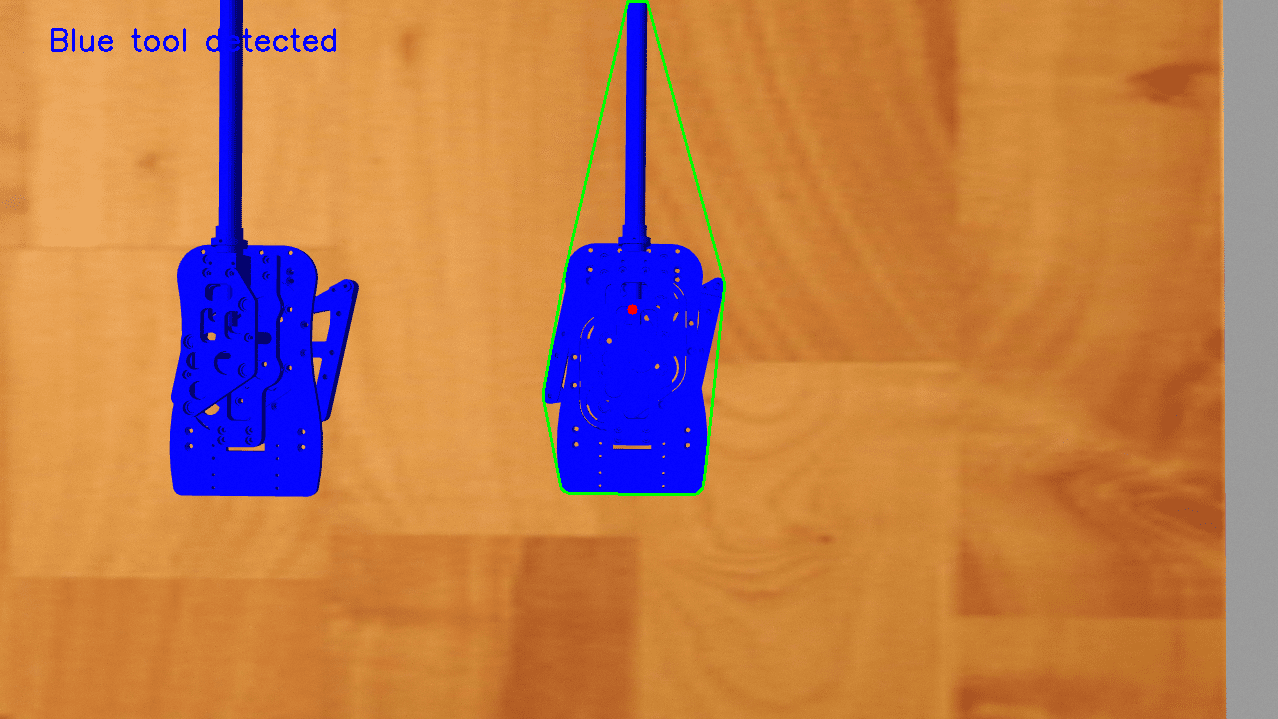
\includegraphics[width=12cm]{images/opencv-tool-convex-hull.png}\\
\caption{Simple tool detection in simulation based on color, using OpenCV. The green polygon is the convex hull, and the red point is the
estimated center of mass}
\end{figure}
\end{center}

\subsection{Stereoscopic vision}

\begin{center}
\begin{figure}[H]
\centering
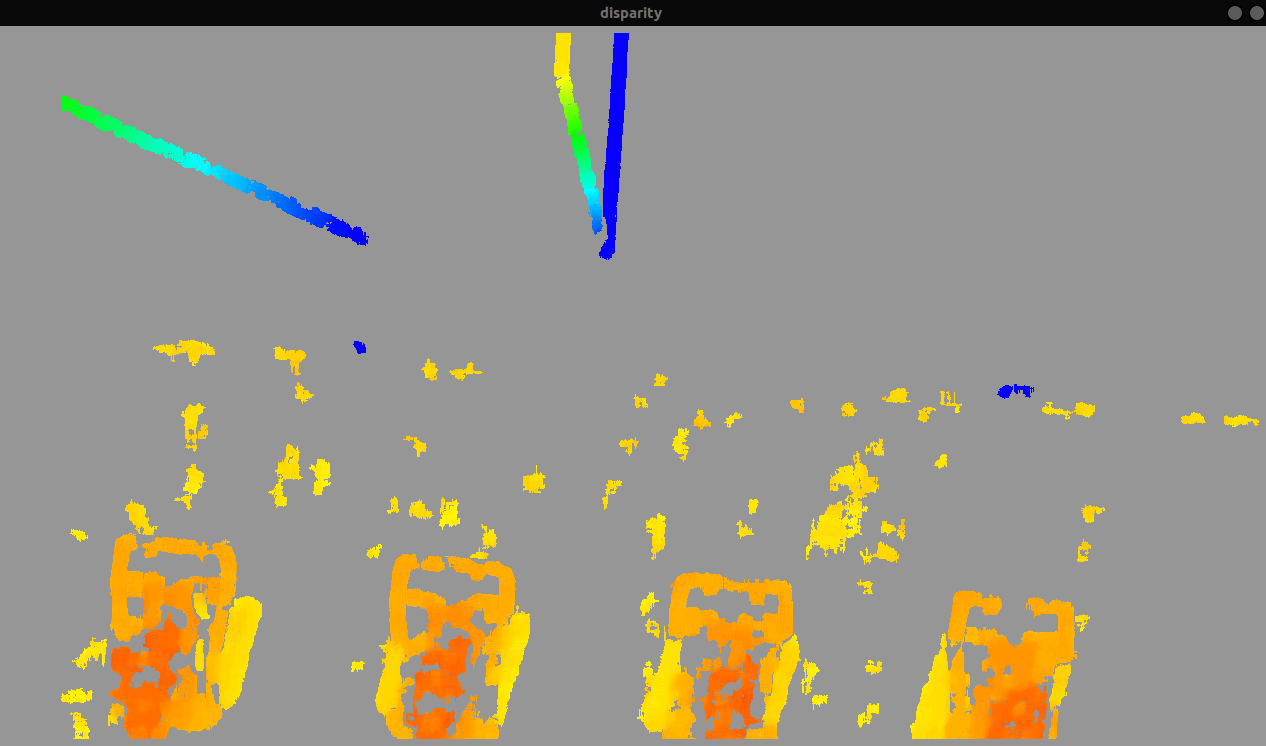
\includegraphics[width=12cm]{images/disparity.png}\\
\caption{Disparity image calculated from the 2 cameras}
\end{figure}
\end{center}

\begin{center}
\begin{figure}[H]
\centering
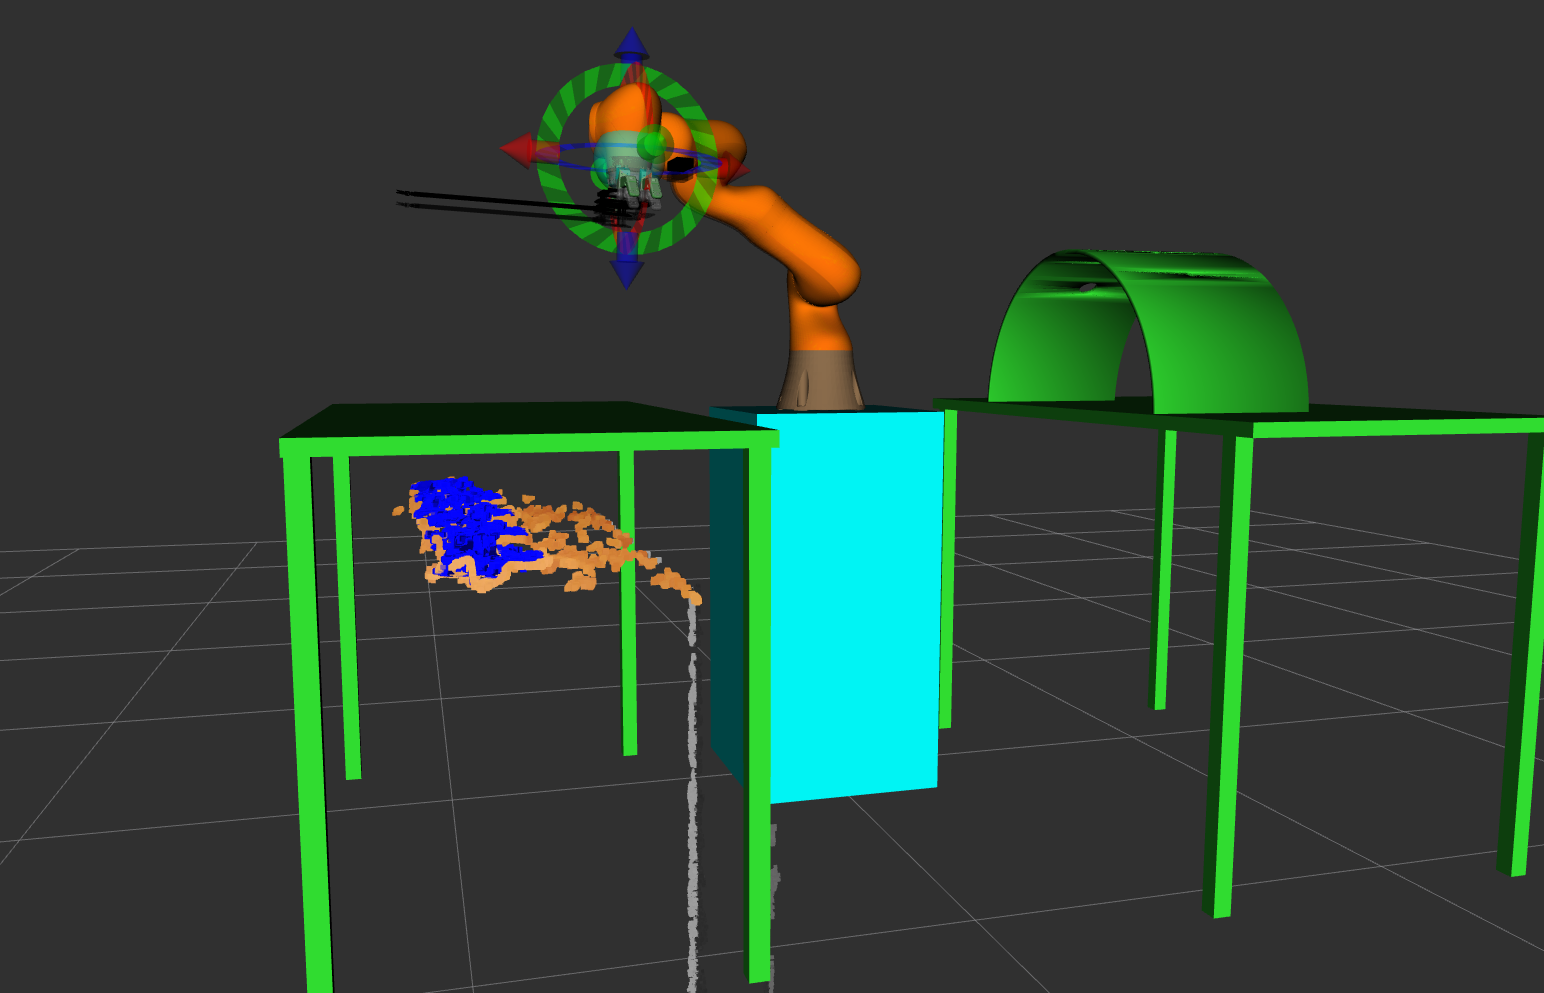
\includegraphics[width=12cm]{images/point_cloud.png}\\
\caption{Point cloud of surgical tools, generated from the 2 cameras and visualized in RViz}
\end{figure}
\end{center}

\subsection{Calculation of tool position and orientation}

In order for the gripper to grasp correctly the laparoscopic tool, it is required to calculate the tool's position and orientation in the pixel space 
which must then be converted with respect to the robot's workspace. From all the pixels that have been classified as part of the laparoscopic tool, 
one can estimate the center of mass and two perpendicular vectors 
attached to that point that define the orientation. The center of mass is simply the average of the $(x,y)$ coordinates of all the tool's pixels
\[
\left( \bar{x}, \bar{y} \right) = \left( \frac{1}{N}\sum_{i=1}^{N} x_i , \frac{1}{N}\sum_{i=1}^{N} y_i \right)
\]

The easiest way to calculate the center of mass is by calculating the average using the first moments of the contour points. However, since the contour is only using
the boundary of the object and not it's area, this method is not very accurate. To get a more accurate value for the center of mass, one must use the pixels that are inside 
the detected object's contour. The simplest way (but most expensive) to get the inside pixels of the tool is to loop over all the pixels and for each pixel check if it is inside the 
polygon (point inside polygon test). To make this method even faster, one can take a sample of the total pixels, for example check one in every 10 pixels in the x and y coordinates, 
which means reducing the time complexity to one tenth. \\

Taking this approach a step further in optimization, one can iterate not in all the video frame pixels but only those pixels 
that are inside the \textbf{Region of Interest} of the tool. The Region of Interest, also known as ROI, is a widely used structure in computer vision and is simply a bounding box (rectangle) that fits exactly 
(or is a bit bigger than) an object or part of the image frame that we want to study. Having already calculated the contour of the surgical tool and it's convex hull we can easily calculate this bounding box. 
For this calculation we prefer to use the convex hull, because it often contains much less pixels than the contour. We iterate over all the pixels of the convex hull and we get the minimum and maximum x and y 
coordinates. The combination of these four values is the desired ROI. Since we now have access to the tool's ROI, we can iterate and sample the pixels inside it (and not all pixels as we did before) to get 
some of the pixels of the tool so that we can more accurately calculate it's center of mass and orientation vectors. \\

The two orientation vectors are the eigenvectors of the covariance matrix of the above pixels. Let $\mathbf{a},\mathbf{b}$ be the orientation vectors, 
then $\mathbf{a},\mathbf{b}$ are solutions of the equation
\[
C \mathbf{v} = λ \mathbf{v}
\]
where $C$ is the covariance matrix given by
\[
C = \begin{bmatrix}
σ(x,x) & σ(x,y) \\
σ(y,x) & σ(y,y) \\
\end{bmatrix}
\]
\[
σ(x,y) = \frac{1}{n-1} \sum_{i=1}^{N} ( x_i - \bar{x} )( y_i - \bar{y} )
\]

\begin{center}
\begin{figure}[H]
\centering
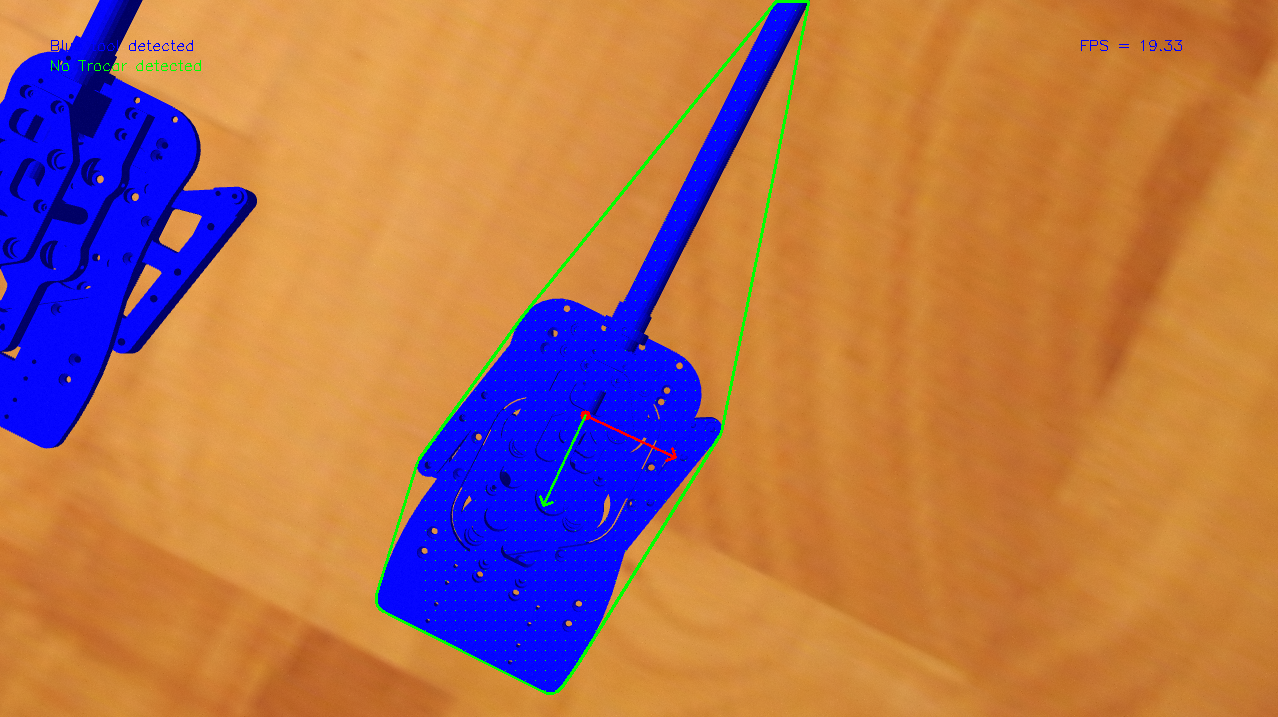
\includegraphics[width=0.8\textwidth]{images/tool-pose.png}\\
\caption{Estimation of tool's pose (position and orientation). The red dot is the center of mass and attached to that are the two orientation vectors of the tool. The green polygon is the convex hull of the tool 
and the white rectangle is it's ROI as calculated from the convex hull}
\end{figure}
\end{center}

\subsection{Calculation of grasping points}

\subsection{Trocar detection \& Estimation of fulcrum point}

\begin{center}
\begin{figure}[H]
\centering
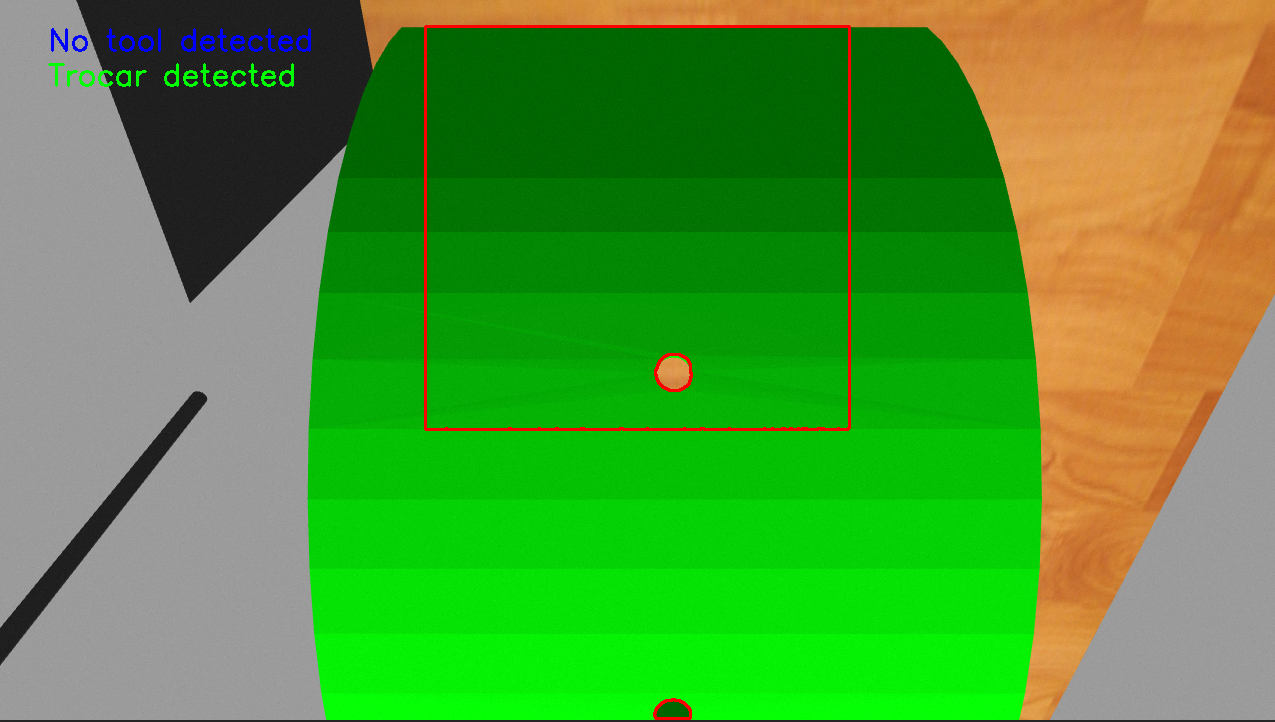
\includegraphics[width=12cm]{images/opencv-trocar-detection.png}\\
\caption{Simple trocar detection in simulation based on color, using OpenCV. In simulation, the trocar is simply considered to be a small 
cylindrical hole and it's center is the fulcrum point}
\end{figure}
\end{center}

\subsection{Visual Servoing}

At this chapter we briefly investigate how visual servoing can be applied in surgery robotics. \textbf{Visual Servoing} is the use of visual information 
to guide and control a robot. The main task of visual servoing is to control the end-effector's pose using features extracted from visual information. The 
features that are usually extracted from cameras are the position and orientation of the detected object, the distance of the object from the camera (using 
stereoscopic vision, photogrammetry or other techniques), the size and the shape of the object. The visual servoing can be executed either in the robot's space 
using position-based servoing or in the camera's space (also known as "pixel space") by using the image-based technique.

\subsubsection{Position based servoing}

\begin{center}
\begin{figure}[H]
\centering
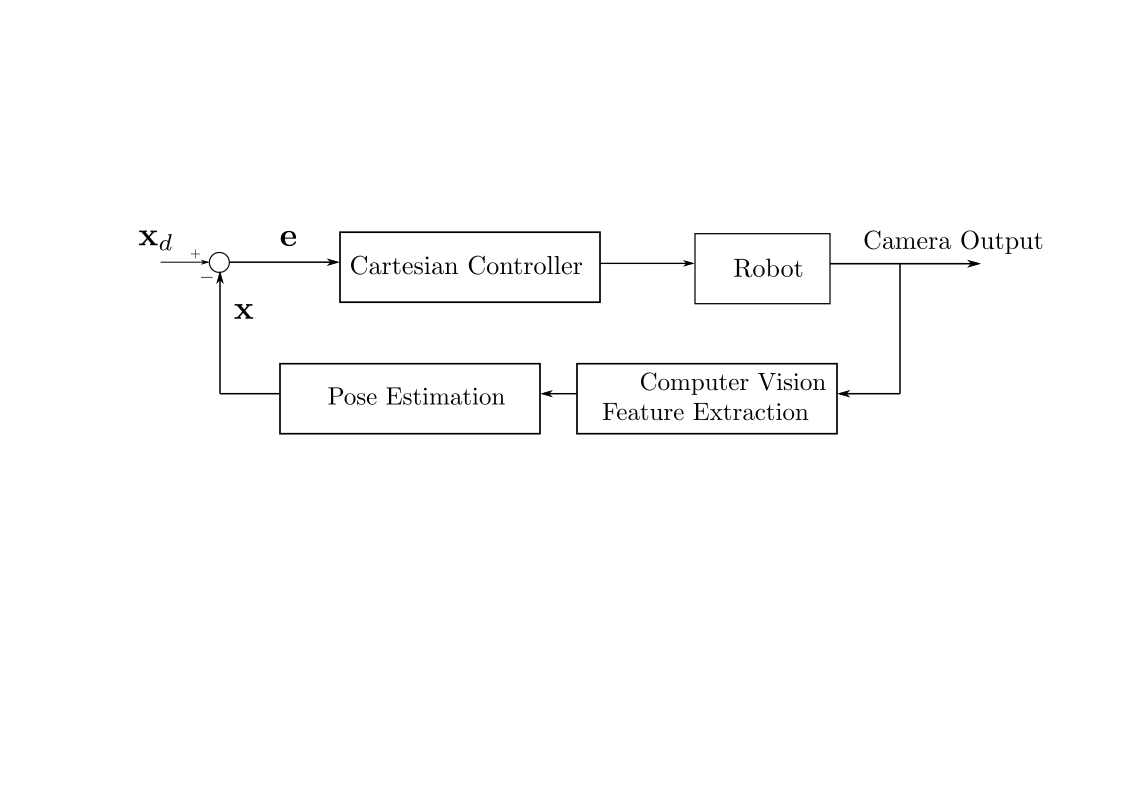
\includegraphics[width=0.8\textwidth]{images/visual-servoing-position-based.png}\\
\caption{Position based visual servoing closed loop control}
\end{figure}
\end{center}

\begin{itemize}
\item \textbf{Photogrammetric technique}
\item \textbf{Stereoscopic vision}
\item \textbf{Extracting depth from motion}
\end{itemize}

\subsubsection{Image based servoing}

\begin{center}
\begin{figure}[H]
\centering

\includegraphics[width=0.8\textwidth]{images/visual-servoing-image-based.png}\\
\caption{Image based visual servoing closed loop control}
\end{figure}
\end{center}

\begin{center}
\begin{figure}[H]
\centering
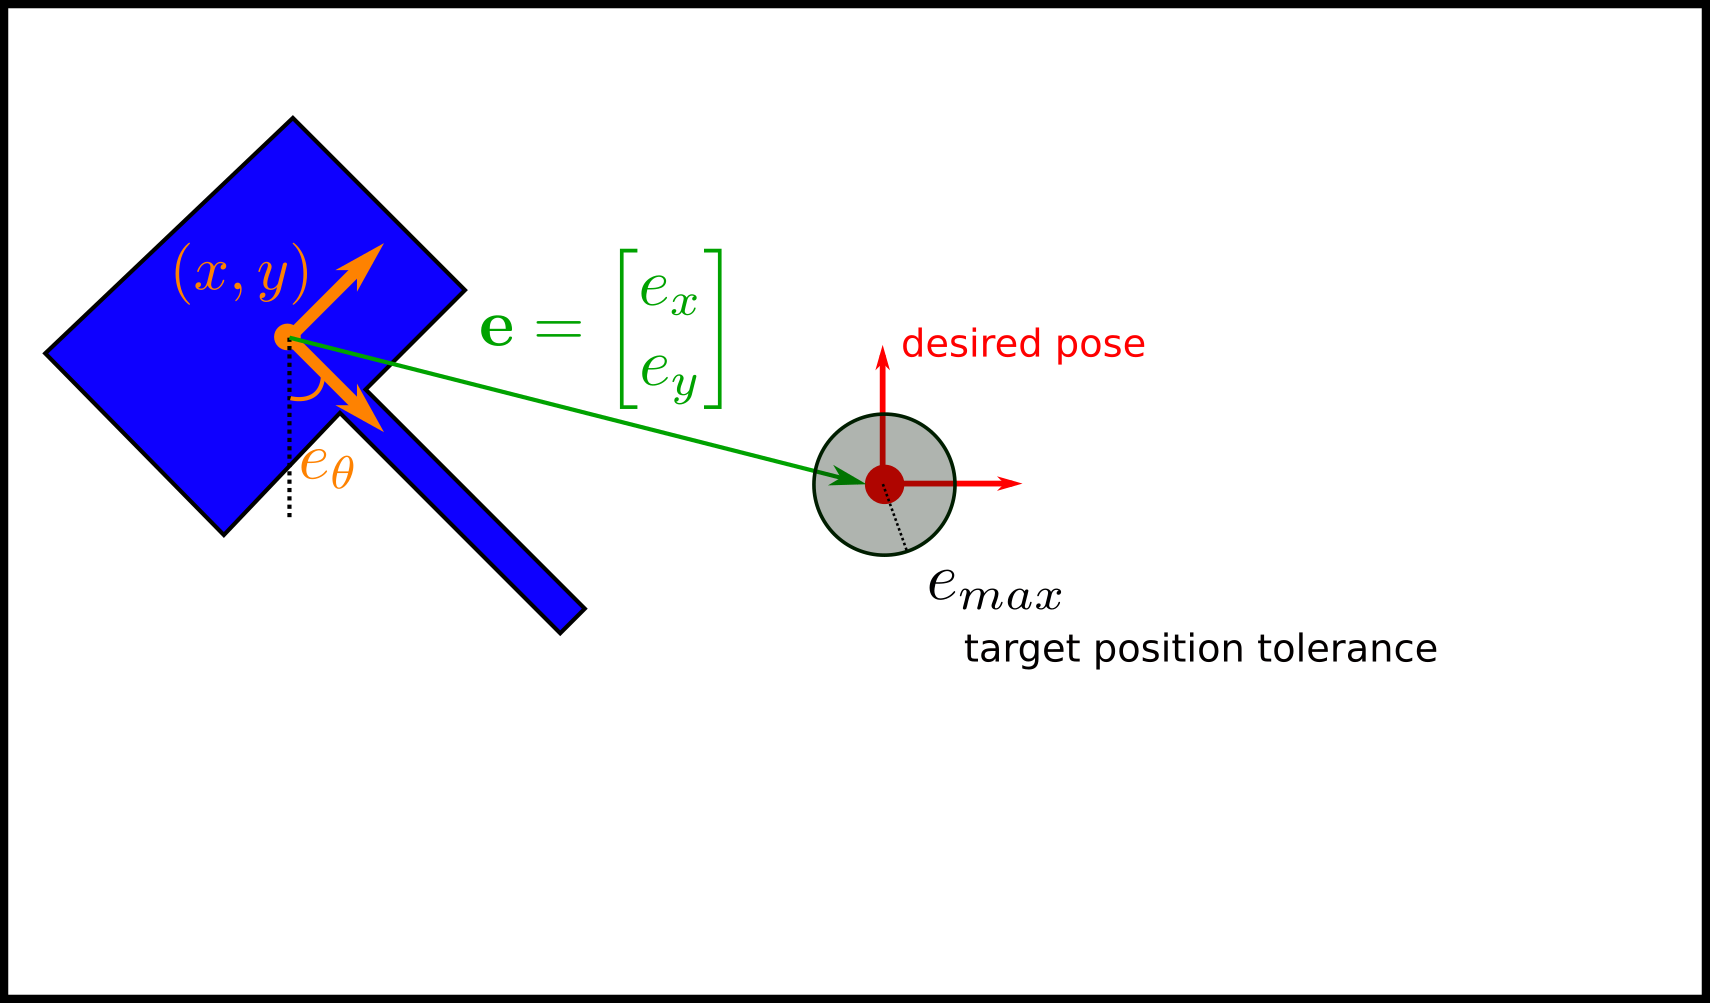
\includegraphics[width=0.45\textwidth]{images/visual_servo_start.png}
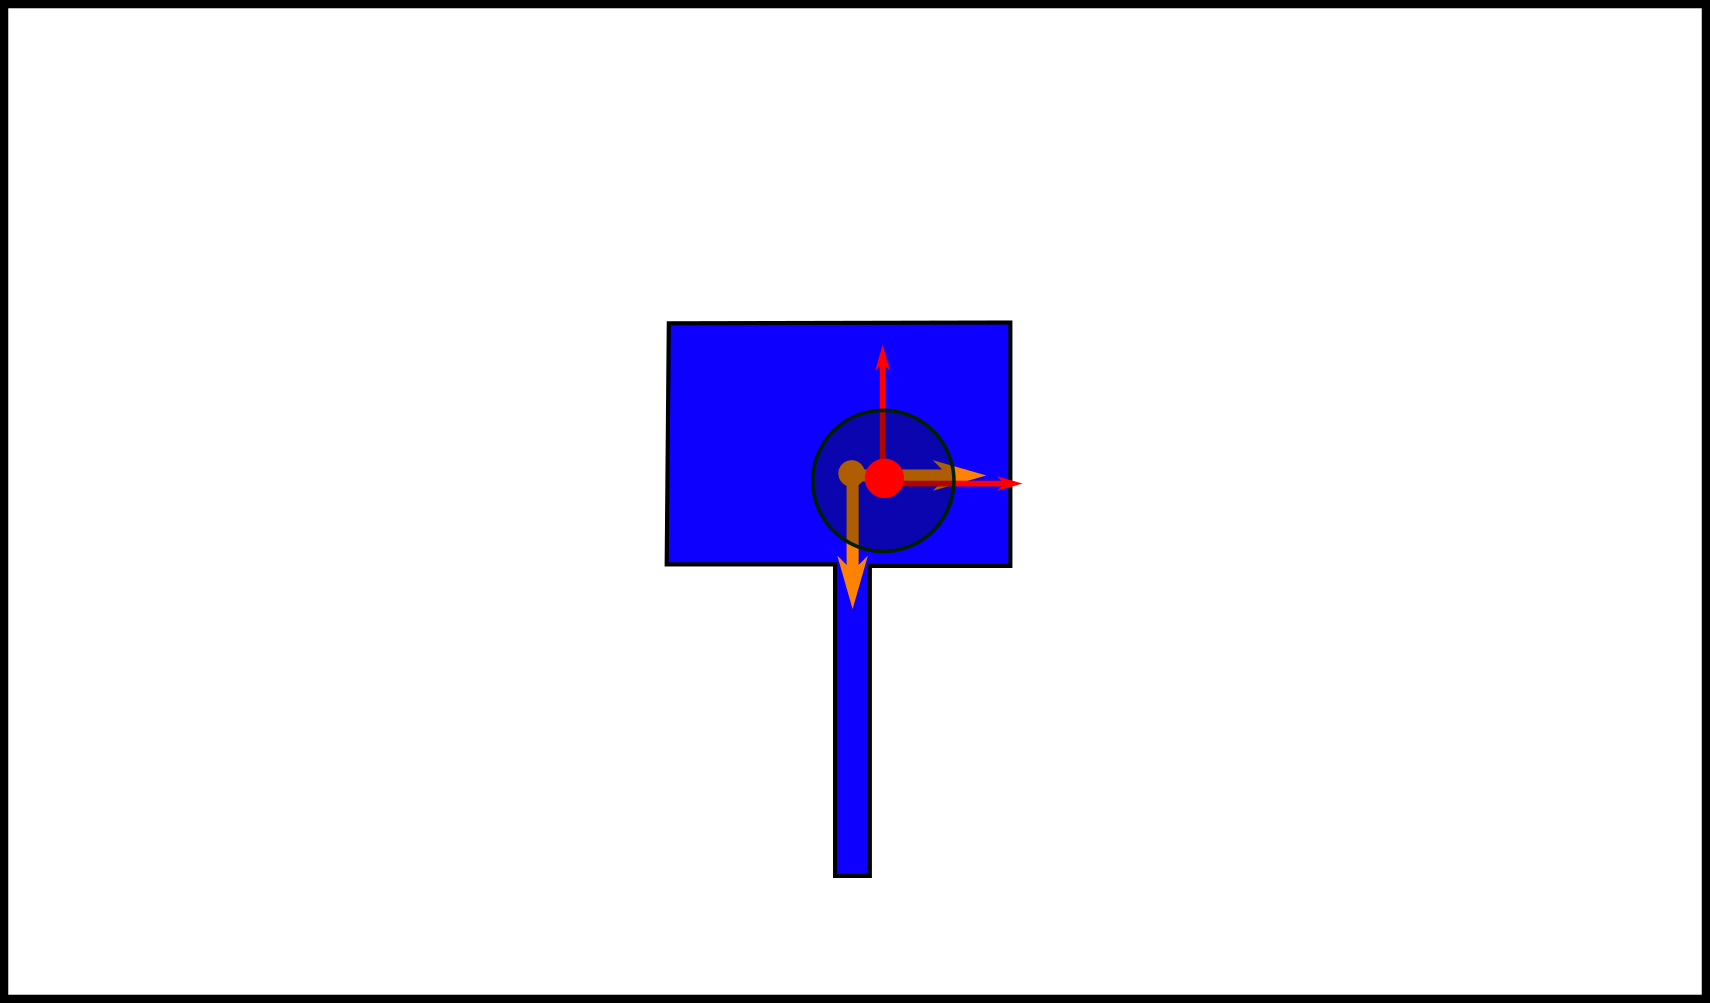
\includegraphics[width=0.45\textwidth]{images/visual_servo_end.png}\\
\caption{Image based visual servoing. The robot arm is controlled using the information gained from the video frames. The frames are 2Dimensional and thus 
the detected objects can have only 3 degrees of freedom which means we can mainly control 3 independent variables, here the $x,y,θ$ variables. The left image 
is the initial frame and the right image is the frame where the object is at the target pose.}
\end{figure}
\end{center}
